\subsection{Orthogonal Matrices}\label{subsec:Orthogonal_Matrices}
There is a particular class of matrices that is very helpful, nice to work with, and has an interesting property.
This is an \nameref{def:Orthogonal_Matrix}.

\begin{definition}[Orthogonal Matrix]\label{def:Orthogonal_Matrix}
  An \emph{orthogonal matrix} is a \nameref{def:Matrix} that is made up of \nameref{def:Orthonormal_Set}s.
  Such a matrix, has the property shown in \Cref{eq:Orthogonal_Matrix_Property}.

  \begin{equation}\label{eq:Orthogonal_Matrix_Property}
    \Transpose{A} = A^{-1}
  \end{equation}
\end{definition}

\begin{definition}[Orthonormal Set]\label{def:Orthonormal_Set}
  An \emph{orthonormal set} is one whose members have unit length (i.e.\ $1$), and whose members are \nameref{def:Linearly_Independent}.

  \begin{remark}
    This is a combination of an orthogonal set and a normal set.
    \begin{description}[noitemsep]
    \item[Orthogonal] The set's component elements are \nameref{def:Linearly_Independent}.
      For vectors (single-column/row matrices), this can be proven by performing the dot product operation on each vector and verifying that it is equal to 0.
    \item[Normal] The set's component elements have a magnitude (vector magnitude in this case) of $1$.
    \end{description}
  \end{remark}
\end{definition}

To show that an \nameref{def:Orthogonal_Matrix} \textbf{requires} \nameref{def:Orthonormal_Set}s, take a small example.

\begin{blackbox}
  Let $A$ be an \nameref{def:Orthogonal_Matrix}.
  Define $A_{n \by 1}$, as:
  \begin{equation*}
    A =
    \begin{pmatrix}
      r_{1} \\ r_{2} \\ \vdots \\ r_{n}
    \end{pmatrix}
  \end{equation*}

  Then,
  \begin{equation*}
    \Transpose{A} =
    \begin{pmatrix}
      r_{1} & r_{2} & \cdots & r_{n}
    \end{pmatrix}
  \end{equation*}

  By the definition of an \nameref{def:Orthogonal_Matrix} and \nameref{def:Inverse_Matrix}, we know that $A \Transpose{A} = I$.
  This means that when multiplying these two matrices together on the $i$th row and $j$th column, we have 2 cases:
  \begin{equation*}
    A_{i \by 1} \Transpose{A}_{1 \by j} =
    \begin{cases}
      1 & \text{ when } i = j \\
      0 & \text{ when } i \neq j
    \end{cases}
  \end{equation*}

  This means that:
  \begin{description}[noitemsep]
  \item When $i \neq j$, then $r_{i} \perp r_{j}$.
  \item When $i = j$, then $r_{i} \Transpose{r_{j}} = 1$, meaning each row has unit length.
  \end{description}
\end{blackbox}

\begin{example}[Lecture 19, Example 3]{Verify Orthogonal Matrix}
  Verify that $A$ is an \nameref{def:Orthogonal_Matrix}?
  \begin{equation*}
    A =
    \begin{pmatrix}
      \frac{2}{3} & \frac{2}{3} & \frac{-1}{3} \\
      \frac{-1}{3} & \frac{2}{3} & \frac{2}{3} \\
      \frac{2}{3} & \frac{-1}{3} & \frac{2}{3}
    \end{pmatrix}
  \end{equation*}
  \tcblower{}
  Start by verifying the magnitude of each row.
  \begin{align*}
    \Magnitude{r_{1}} &= \sqrt{{(\frac{2}{3})}^{2} + {(\frac{2}{3})}^{2} + {(\frac{-1}{3})}^{2}} \\
                      &= \sqrt{\frac{4}{9} + \frac{4}{9} + \frac{1}{9}} \\
                      &= \sqrt{1} \\
                      &= 1
  \end{align*}
  Realistically, we should verify $\Magnitude{r_{2}} = 1$ and $\Magnitude{r_{3}} = 1$.
  However, because their numbers are the same, their magnitude will be the same.
  Thus, the sets are normal.

  Now, check if the sets are orthogonal.
  \begin{align*}
    r_{1} \cdot r_{2} &= \frac{-2}{9} + \frac{4}{9} - \frac{2}{9} \\
                     &= 0
  \end{align*}
  Realistically, we should verify $r_{2} \cdot r_{3} = 0$ and $r_{1} \cdot r_{3} = 0$.
  However, because their numbers are the same, their results will be the same.
  Thus, the sets are orthogonal.

  $\therefore$ $A$ is an \nameref{def:Orthogonal_Matrix}.
\end{example}

\subsubsection{Quadratic Forms}\label{subsubsec:Quadratic_Forms}
We can use a \nameref{def:Real_Symmetric_Matrix} to represent a \nameref{def:Quadratic_Form}.

\begin{definition}[Real Symmetric Matrix]\label{def:Real_Symmetric_Matrix}
  A \emph{real, symmetric matrix} is a matrix whose non-diagonal elements are mirrored across the diagonal.
  For example:
  \begin{equation*}
    \begin{pmatrix}
      1 & 3 & 5 \\
      3 & 28 & 7 \\
      5 & 7 & 15 \\
    \end{pmatrix}
  \end{equation*}
\end{definition}

A real symmetric matrix has two important properties.
\begin{propertylist}
\item The \nameref{def:Eigenvalue}s of the matrix are real ($\in \RealNumbers$).\label{prop:Real_Symmetric_Matrix-Real_Eigenvalues}
\item \nameref{def:Eigenvector}s corresponding to \textbf{distinct} \nameref{def:Eigenvalue}s are orthogonal to each other.\label{prop:Real_Symmetric_Matrix-Distinct_Eigenvectors}
\end{propertylist}

\begin{definition}[Quadratic Form]\label{def:Quadratic_Form}
  A \emph{quadratic form} is a polynomial equation.
  We can use a \nameref{def:Real_Symmetric_Matrix} and \nameref{def:Diagonalization} to turn the polynomial into a real symmetric matrix that we can then use to yield a conic section in the Cartesian plane.

  For our purposes, we choose to say $a, b, c \in \RealNumbers$.
  \begin{equation}\label{eq:Quadratic_Form}
    ax_{1}^{2} + 2bx_{2} + c =
    \begin{pmatrix}
      x_{1} & x_{2}
    \end{pmatrix}
    \begin{pmatrix}
      a & b \\
      b & c
    \end{pmatrix}
    \begin{pmatrix}
      x_{1} \\ x_{2}
    \end{pmatrix}
  \end{equation}

  \begin{remark}[Complex Quadratic Form]\label{rmk:Complex_Quadratic_Form}
    A \nameref{def:Quadratic_Form} may be complex if $a$, $b$, or $c$ are complex.
    These can be solved in a similar fashion, but must be done with a \nameref{def:Hermitian_Matrix} instead.
  \end{remark}
\end{definition}

\begin{example}[Lecture 20, Example 2]{Classify Conic Section}
  Classify the conic section produced by the \nameref{def:Quadratic_Form} shown below?
  In addition, sketch it, and determine its principle axes?
  \begin{equation*}
    4x_{1}^{2} + 8x_{1}x_{2} - 2x_{2}^{2} = 24
  \end{equation*}
  \tcblower{}
  First thing we must do is convert the \nameref{def:Quadratic_Form} into a series of matrices.
  \begin{align*}
    \begin{pmatrix}
      x_{1} & x_{2}
    \end{pmatrix}
              \begin{pmatrix}
                4 & 4 \\
                4 & -2
              \end{pmatrix}
                    \begin{pmatrix}
                      x_{1} \\ x_{2}
                    \end{pmatrix} &= 24 \\
    \Transpose{X} A X &= 24
  \end{align*}

  Now, we want a way to simplify $A$ such that we have an easy conic section to work with.
  In this case, $D$, the \nameref{def:Diagonal_Matrix} of $A$ will provide us with such a simplification.
  Thus, we must find the \nameref{def:Eigenvalue}s, \nameref{def:Eigenvector}s, and ensure the $P$ created is \nameref{def:Orthogonal_Matrix}.
  \begin{align*}
    A - \lambda I &=
                    \begin{pmatrix}
                      4 - \lambda & 4 \\
                      4 & -2 - \lambda
                    \end{pmatrix} \\
    \det(A - \lambda I) &= (4 - \lambda) (-2 - \lambda) - 4 (4) \\
                  &= \lambda^{2} - 2 \lambda - 24 \\
                  &= (\lambda - 6) (\lambda + 4)
  \end{align*}

  We get \nameref{def:Eigenvalue}s if and only if $\det(A-\lambda I) = 0$.
  So, the two eigenvalues are: $\lambda = 6$ and $\lambda = -4$, both with algebraic multiplicity 1.

  Starting with $\lambda = 6$:
  \begin{align*}
    A - \lambda I &=
                    \begin{pmatrix}
                      -2 & 4 \\
                      4 & -8
                    \end{pmatrix} \\
    \begin{pmatrix}
      -2 & 4 \\
      4 & -8
    \end{pmatrix}
          \begin{pmatrix}
            x_{1} \\ x_{2}
          \end{pmatrix} &=
                          \begin{pmatrix}
                            0 \\ 0
                          \end{pmatrix} \\
    \intertext{Converting the matrix equation to a system of linear equations.}
    -2x_{1} + 4x_{2} &= 0 \\
    4x_{1} - 8x_{2} &= 0 \\
    \intertext{Solving the system.}
    x_{1} &= 2 x_{2} \\
    x_{2} &= x_{2} \\
    \intertext{Putting the solutions found back into the variable matrix.}
    \begin{pmatrix}
      x_{1} \\ x_{2}
    \end{pmatrix} &=
                    \begin{pmatrix}
                      2 x_{2} \\ x_{2}
                    \end{pmatrix} \\
    &= x_{2}
      \begin{pmatrix}
        2 \\ 1
      \end{pmatrix}
  \end{align*}

  Thus, the \nameref{def:Eigenvector} for the \nameref{def:Eigenvalue} $\lambda = 6$ is:
  \begin{equation*}
    = x_{2}
    \begin{pmatrix}
      2 \\ 1
    \end{pmatrix}\text{, where } x_{2} \neq 0
  \end{equation*}

  Now, $\lambda = -4$:
  \begin{align*}
    A - \lambda I &=
                    \begin{pmatrix}
                      8 & 4 \\
                      4 & 2
                    \end{pmatrix} \\
    \begin{pmatrix}
      8 & 4 \\
      4 & 2
    \end{pmatrix}
          \begin{pmatrix}
            x_{1} \\ x_{2}
          \end{pmatrix} &=
                          \begin{pmatrix}
                            0 \\ 0
                          \end{pmatrix} \\
    \intertext{Converting the matrix equation to a system of linear equations.}
    8x_{1} + 4x_{2} &= 0 \\
    4x_{1} + 2x_{2} &= 0 \\
    \intertext{Solving the system.}
    x_{1} &= \frac{-1}{2} x_{2} \\
    x_{2} &= x_{2} \\
    \intertext{Putting the solutions found back into the variable matrix.}
    \begin{pmatrix}
      x_{1} \\ x_{2}
    \end{pmatrix} &=
                    \begin{pmatrix}
                      \frac{-1}{2} x_{2} \\ x_{2}
                    \end{pmatrix} \\
    &= x_{2}
      \begin{pmatrix}
        \frac{-1}{2} \\ 1
      \end{pmatrix}
  \end{align*}

  Thus, the \nameref{def:Eigenvector} for the \nameref{def:Eigenvalue} $\lambda = 6$ is:
  \begin{equation*}
    = x_{2}
    \begin{pmatrix}
      \frac{-1}{2} \\ 1
    \end{pmatrix}\text{, where } x_{2} \neq 0
  \end{equation*}

  Double-checking that the distinct \nameref{def:Eigenvector}s are orthogonal, we perform the dot product.
  From the definition of an \nameref{def:Eigenvector}, we are allowed to scale the base vector by any scalar value, and the new vector remains an eigenvector of the original matrix.
  In this case, scaling the \nameref{def:Eigenvector} corresponding to $\lambda = -4$ by 2, we remove the fraction, simplifying our calculations.
  \begin{align*}
    \begin{pmatrix}
      2 \\ 1
    \end{pmatrix} \cdot
    \begin{pmatrix}
      -1 \\ 2
    \end{pmatrix} &= 2 (-1) + 1 (2) \\
                  &= -2 + 2 \\
                  &= 0
  \end{align*}
  $\therefore$ the two eigenvectors are orthogonal.

  Now, we need to normalize the vectors.
  \begin{align*}
    \Magnitude{c_{1}} &= \sqrt{2^{2} + 1^{2}} \\
                      &= \sqrt{4 + 1} \\
                      &= \sqrt{5} \\
    \intertext{Similarly, the magnitude of the second column is the same.}
  \end{align*}

  So, an \nameref{def:Orthogonal_Matrix} $P$ is:
  \begin{equation*}
    P =
    \begin{pmatrix}
      \frac{2}{\sqrt{5}} & \frac{-1}{\sqrt{5}} \\
      \frac{1}{\sqrt{5}} & \frac{2}{\sqrt{5}}
    \end{pmatrix}
  \end{equation*}

  Because $P$ is a matrix that implements a \nameref{def:Diagonalization} of $A$, we know $P^{-1} A P = D$.
  This means $A = P D P^{-1}$.
  Also, because $P$ is \nameref{def:Orthogonal_Matrix}, we know $P^{-1} = \Transpose{P}$.
  So, $A = P D \Transpose{P}$, where $D =
  \begin{pmatrix}
    6 & 0 \\
    0 & -4
  \end{pmatrix}$.

  Now, plugging the equivalency we found for $A$ into the converted \nameref{def:Quadratic_Form}, we have:
  \begin{align*}
    \Transpose{X} A X &= 24 \\
    A &= P D \Transpose{P} \\
    \Transpose{X} (P D \Transpose{P}) X &= 24 \\
    \intertext{Matrix multiplication is associative in this way already, so drop the parentheses.}
    \Transpose{X} P D \Transpose{P} X &= 24 \\
  \end{align*}

  Now, we can change the axes of this problem, creating a whole new coordinate system.
  This is done by defining $Y = \Transpose{P} X$.
  The principle axes of this coordinate system can be found by solving:
  \begin{align*}
    X &= t p_{1} & X &= t p_{2} \\
    \begin{pmatrix}
      x_{1} \\ x_{2}
    \end{pmatrix} &= t
                    \begin{pmatrix}
                      \frac{1}{\sqrt{5}} \\ \frac{2}{\sqrt{5}}
                    \end{pmatrix} & \begin{pmatrix}
                      x_{1} \\ x_{2}
                    \end{pmatrix} &= t
                                    \begin{pmatrix}
                                      \frac{-2}{\sqrt{5}} \\ \frac{1}{\sqrt{5}}
                                    \end{pmatrix} \\
    \intertext{Solving each system of equations, we find:}
    x_{2} &= 2x_{1} & x_{2} &= \frac{-1}{2} x_{1}
    \intertext{Due to the way we defined $Y$ earlier, the first equation is the definition of $y_{1}$ in the original coordinate system.
    Likewise for $y_{2}$.}
  \end{align*}

  We defined $Y$ as $Y = \Transpose{P} X$, which means that, according to the properties of matrix transposition, $\Transpose{Y} = \Transpose{X} P$.
  So we now have:
  \begin{align*}
    \Transpose{X} P D \Transpose{P} X &= 24 \\
    \Transpose{Y} D Y &= 24 \\
    \Transpose{Y}
    \begin{pmatrix}
      6 & 0 \\
      0 & -4
    \end{pmatrix} Y &= 24 \\
    \intertext{Using the theory of \nameref{def:Quadratic_Form}s again, we can expand this to a quadratic equation again.}
    6y_{1}^{2} - 4y_{2}^{2} &= 24 \\
    \frac{y_{1}^{2}}{4} - \frac{y_{2}^{2}}{6} &= 1
  \end{align*}

  So, the original \nameref{def:Quadratic_Form} is a hyperbola.
  Roughly sketched, it looks like the figure below.

  \begin{center}
    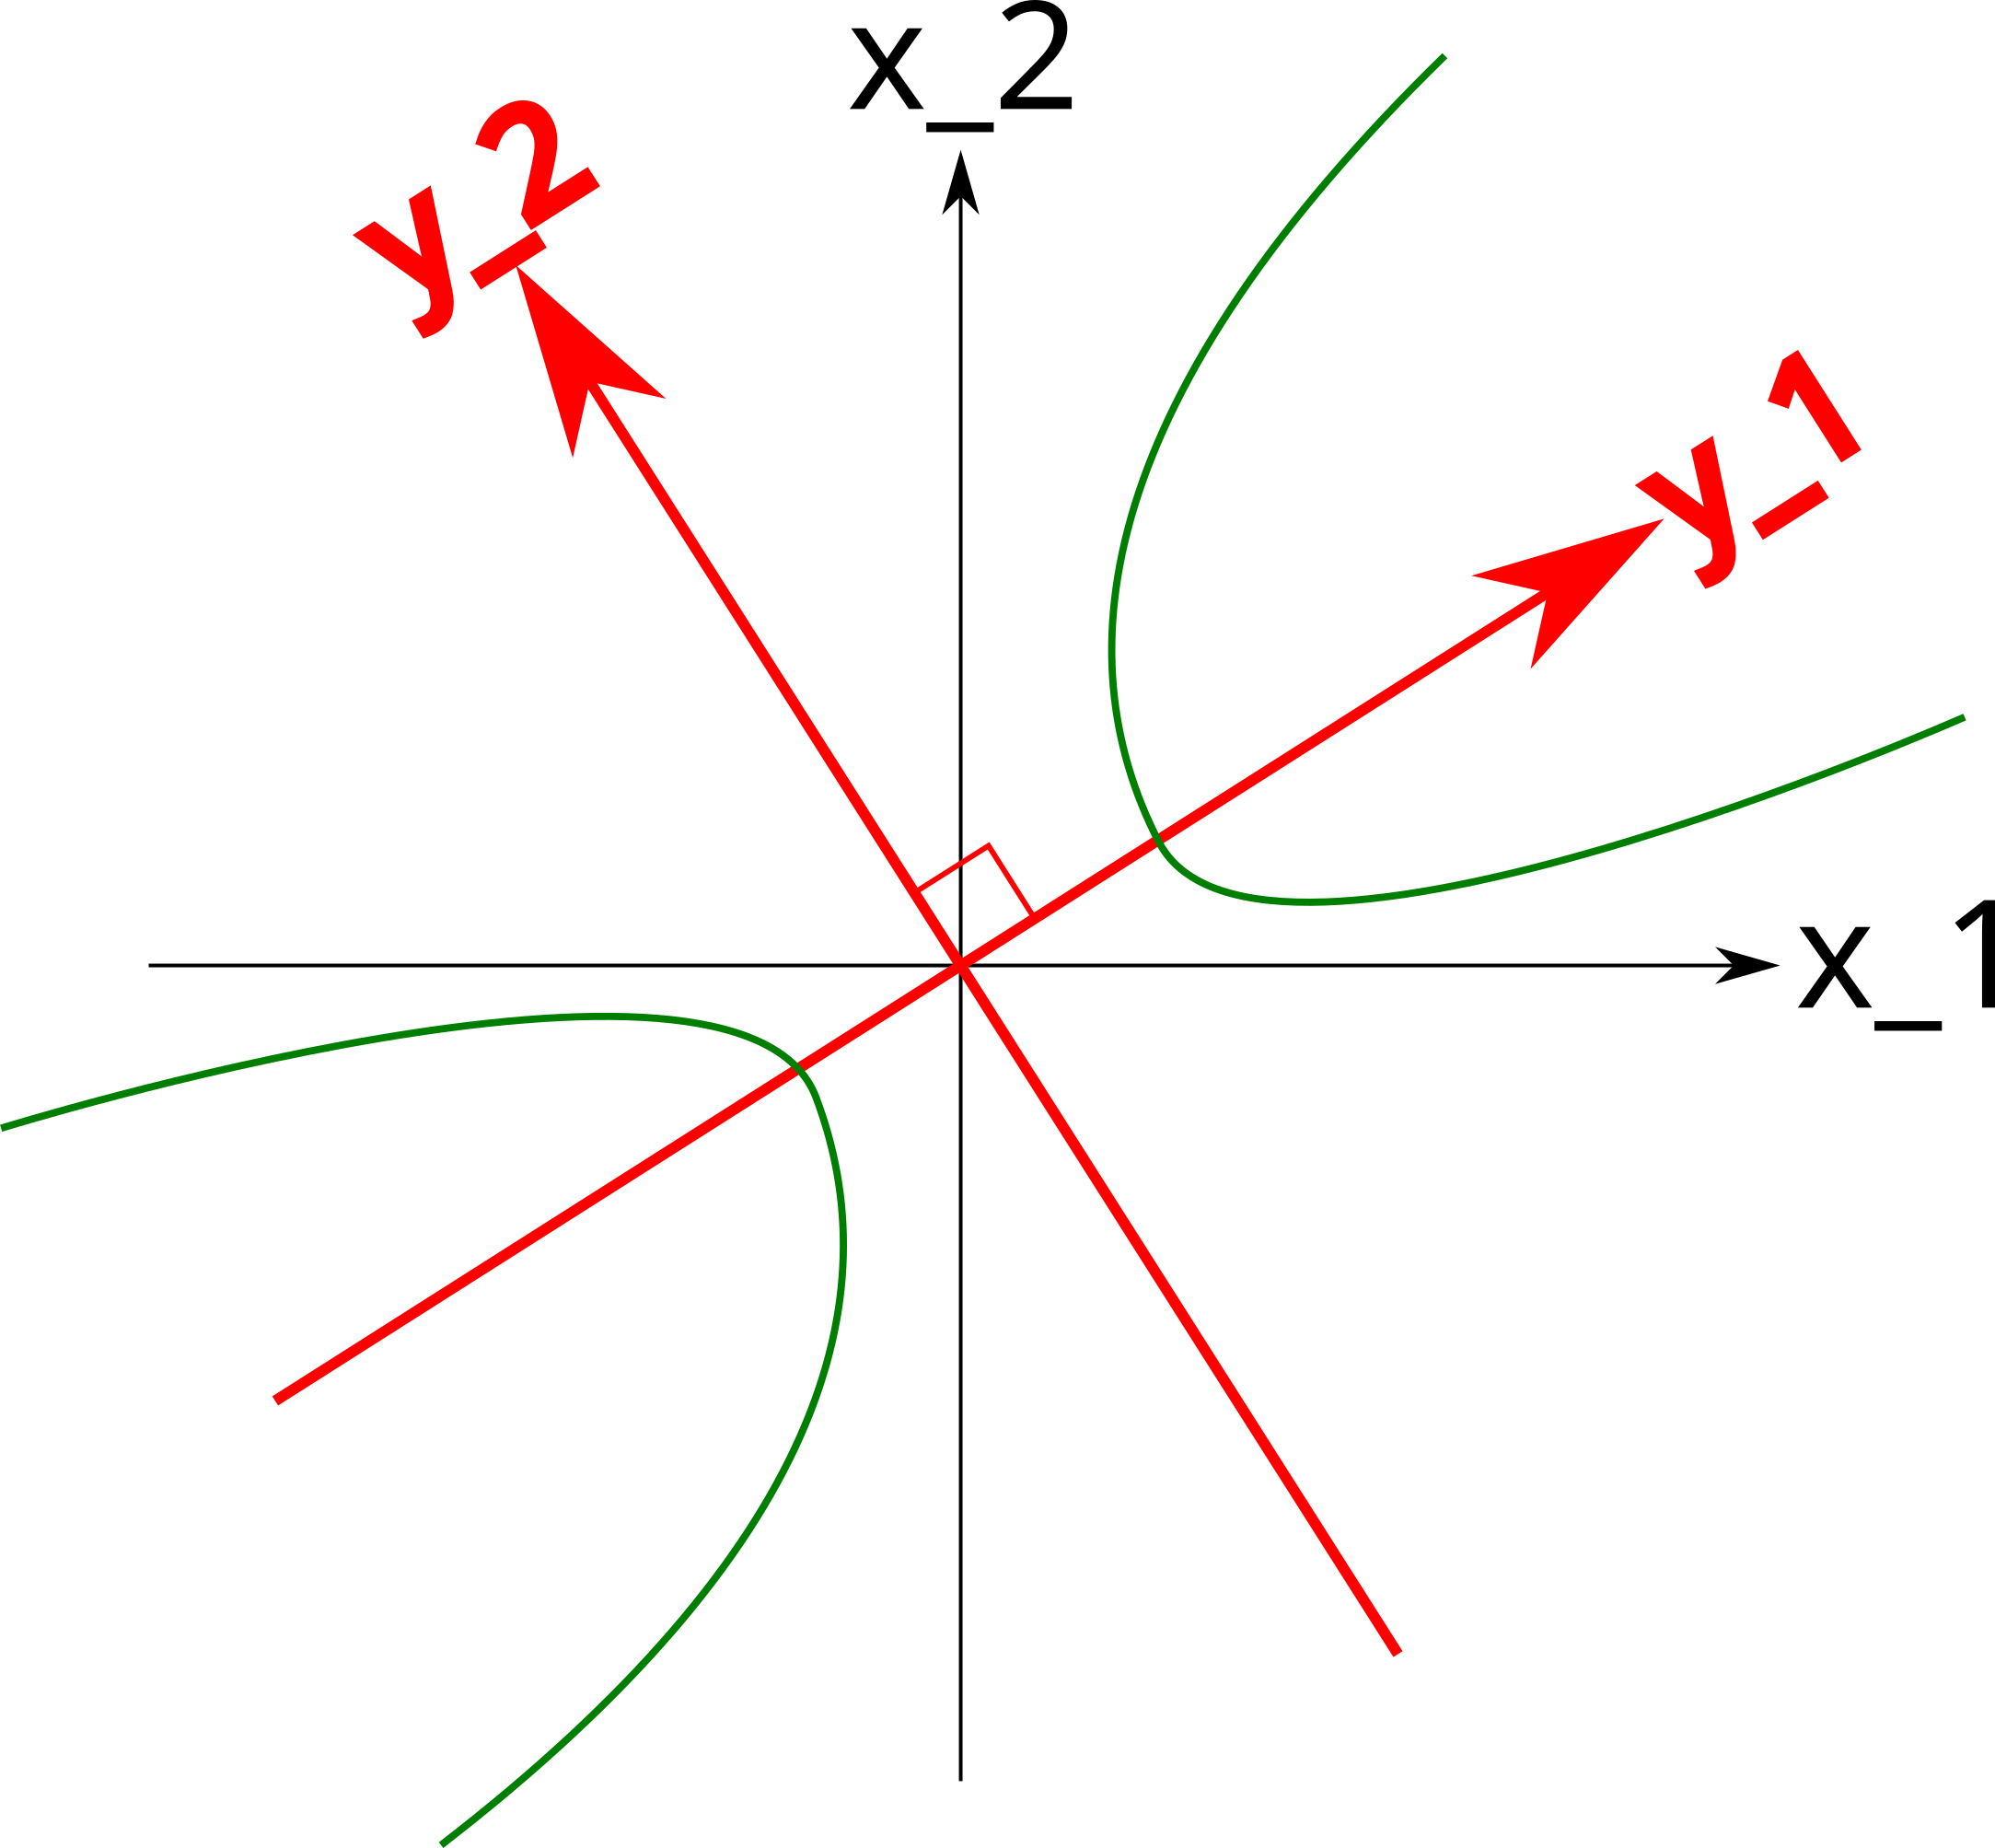
\includegraphics[scale=0.50]{./Quadratic_Form.png}
  \end{center}
\end{example}


%%% Local Variables:
%%% mode: latex
%%% TeX-master: "../../Math_333-MatrixAlg_ComplexVars-Reference_Sheet"
%%% End:
